\section{Geschichte der Ruprecht-Karls-Universität Heidelberg}
\label{geschichte}
Die Ruperto Carola wurde im Jahre 1386 mit päpstlicher Genehmigung von Kurfürst 
Ruprecht I. als Ruprechts-Universität Heidelberg gegründet. Sie ist die Dritte im 
Heiligen römischen Reich deutscher Nation nach Prag und Wien, also die älteste in 
den Grenzen des heutigen Deutschlands. Aufgrund der Spaltung der Kirche war es 
nötig geworden, eine Ausbildung eigener Theologen zu ermöglichen, da 
Sorbonne-Absolventen nicht mehr im römischen Reich in kirchliche Dienste treten durften.
Marsilius von Inghen, der Gründungsrektor, wegen der Kirchenspaltung aus Paris geflohen, eröffnet die Universität im Oktober 1386 mit einer feierlichen Messe. Die Anfänge 
der Universität sind durch erhebliche Raumprobleme gekennzeichnet: Kirchen und 
Klostersäle werden für Vorlesungen genutzt. Erst später können eigene Gebäude für 
die Lehre errichtet werden. Im Zuge der Universitätsgründung werden die 
Stiftsbibliotheken der umliegenden Klöster vereinigt, um eine einigermaßen solide 
Ausbildung zu gewährleisten; die Büchersammlung wird dabei kontinuierlich erweitert 
(zum Beispiel durch vererbte Bestände der Augsburger Handelsfamilie Fugger) und im 
16. Jahrhundert zur Bibliotheca Palatina vereinigt.

1556 wird die Universität im Zuge der Reformation in eine evangelische 
Landeshochschule umgewandelt. Kurfürst Ottheinrich führt normale bürgerliche 
Kleidung statt der sonst üblichen geistlichen Tracht für Studierende ein. Auch die 
finanzielle Situation verbessert sich stark durch die Übertragung von Kirchengut an 
die Universität. Später wird die Universität sogar als calvinistische Hochschule im 
„deutschen Genf“ bezeichnet. So blüht sie bis 1618 auf, die Studierendenzahlen wachsen, 
auch wenn die Universität im Vergleich zu anderen deutschen Universitäten immer noch 
zu den kleinen zählt.
\marginpar{
    \centering{
        \vspace{-50mm}
        
\includegraphics[width=3cm]{bilder/a_wise_man_once_said_1.PNG}\\\vspace{13mm}
        
\includegraphics[width=3cm]{bilder/a_wise_man_once_said_2.PNG}\\\vspace{13mm}
        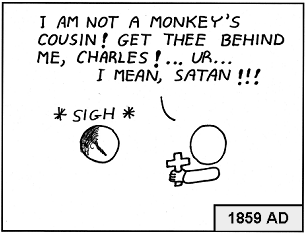
\includegraphics[width=3cm]{bilder/a_wise_man_once_said_3.PNG}\\\vspace{13mm}
        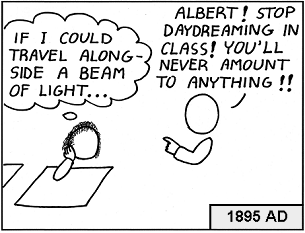
\includegraphics[width=3cm]{bilder/a_wise_man_once_said_4.PNG}\\\vspace{13mm}
        
\includegraphics[width=3cm]{bilder/a_wise_man_once_said_5.PNG}\\\vspace{13mm}
        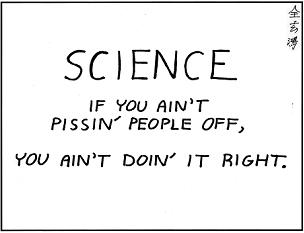
\includegraphics[width=3cm]{bilder/a_wise_man_once_said_6.PNG}\\\vspace{13mm}
    }
}



Während des 30-jährigen Kriegs wird die Universität ziemlich stark beschädigt und 
der Lehrbetrieb muss immer wieder unterbrochen werden bis sie schließlich 1652 
wiedereröffnet wird. Doch der Frieden hält nicht lange an. Im Zuge des Pfälzer 
Erbfolgekrieges wird die ganze Stadt Heidelberg verwüstet. Die Bibliotheca Palatina 
wird als Kriegskostenersatz an den Papst verschenkt. 

%% der lehrbetrieb wurde eingestellt und eigentlich gabs die Uni nicht Davon erholt sich die 
%Universität nur sehr langsam.

Mitte des 18. Jahrhunderts beginnen sich die Naturwissenschaften zu etablieren. 
Zuerst als Teil der philosophischen Fakultät entsteht 1752 der Lehrstuhl für 
Mathematik und Experimentalphysik. Diese Entwicklung setzt sich 1802 mit dem 
Übergang Heidelbergs an Baden fort. Die Universität erweitert nach dem ersten 
Großherzog von Baden ihren Namen zu „Ruprecht-Karls-Universität Heidelberg“. Sie ist 
von jetzt an staatlich finanziert und wird komplett reorganisiert. Die 
Naturwissenschaftlich-Mathematische Fakultät trennt sich von der Philosophischen und 
entwickelt sich vor allem unter dem Einfluss von Robert Bunsen, Gustav Kirchhoff und 
Hermann von Helmholtz. Georg Wilhelm Friedrich Hegel lehrt zwei Jahre an der 
philosophischen Fakultät, die medizinische Fakultät zieht Patienten aus aller Welt an. 
Trotzdem wird Heidelberg vor allem als juristische Universität gesehen. Auch kommt 
es in dieser Zeit zu Entwicklungen in der Frauengleichstellung. Im Jahr 1895 
promoviert Katharina Windscheid als erste Doktorandin in Heidelberg. 1900 wird 
Georgine Sexauer als erste Studentin immatrikuliert und 1923 wird Gerta von Ubisch 
als Professorin für Botanik habilitiert.

Im 20. Jahrhundert setzt sich dieser Trend fort. Heidelberg ist eine weltoffene und 
liberale Universität, an der man auch eine große Zahl von ausländischen Studierenden 
findet. Das interdisziplinäre Gespräch wird gesucht, was der Uni ihren typischen 
„Heidelberger Geist“ verleiht, der in der Weimarer Republik auch häufig als 
demokratischer Geist bezeichnet wird.

Trotzdem wird die Studierendenschaft im Verlauf des 20. Jahrhunderts immer radikaler 
und mit dem Erstarken des Nationalsozialismus werden viele ProfessorenInnen entlassen und 
Studierende aus politischen und rassistischen Gründen ausgeschlossen. Bei der 
Bücherverbrennung auf dem Universitätsplatz 1933 nehmen viele Mitglieder der 
Universität aktiv teil; die Ruperto Carola ist als braune Universität verrufen.
Die Athene wich dem Hakenkreuz, der lebendige Geist dem deutschen. 

Nach dem zweiten Weltkrieg ist die Universität äußerlich zerstört, gravierender sind jedoch die Schäden die durch die nationalsozialistische Ideologie verbleiben. Der inneren Erneuerung widmeten sich maßgeblich Karl Jaspers und Karl Heinrich Bauer, die eine 
neue Satzung ausgearbeitet und in den folgenden Jahren die Universität stark erweitern. 

Trotz aller wissenschaftlichen Erneuerung bleibt das reaktionäre Geflecht an der Universität erhalten - Athene hat ihren Platz zurück erobert, doch der lebendige freie Geist ist nicht zurück gekehrt.
Gegen diese Verkrustungen begehrt die Studierendenbewegung Ende der 60er Jahre auf. Mit der polizeilichen Räumung von besetzten Universitätsgebäuden und Verhaftung von Studierenden findet diese Bewegung in Heidelberg wie auch ganz Deutschland ein jähes Ende. Als Reaktion und Bestrafung wurden studentische Mitbestimmungsrechte massiv beschnitten und seit dem nur teilweise wieder eingeführt (hier fehlt das - Verweis auf HOPO artikel).

Die Universität gewinnt stetig Studierende und wird mit der Erschließung des Neuenheimer Feldes stark erweitert. Bis zum Jubiläumsjahr 1986 wächst die Zahl 
der Studierenden auf ca. 27\,000 an. Heidelberg erarbeitet sich in Deutschland und darüber hinaus einen Ruf als forschungsstarke Universität.





Die neuesten Entwicklungen stammen aus dem Jahr 2007. Seitdem darf sich die 
Universität „Exzellenzuni“ nennen, denn ihr Zukunftskonzept „Heidelberg: Realising 
the Potential of a Comprehensive University“ wurde als förderungswürdig ausgewählt. 
